% \pagenumbering{arabic}
% \setcounter{page}{1}

\chapter{Introduction}
\label{chap:introduction}

\section{Motivation}
\label{sec:motivation}
\indent \indent
Computers have improved almost every aspect of modern life. Recently, home security has become a target of the technology revolution. Companies like Ring \cite{RING} and Eufy \cite{EUFY} offer IoT devices like doorbells and cameras to allow their customers to continuously monitor their property. On top of traditional surveillance, these companies also provide software solutions to analyse footage. For example, a doorbell may recognise a visitor or alert to the presence of a stranger. However, the computational intensity of inference means footage must be transferred to more powerful servers. 
\smallskip \\ \indent
To provide security, video is encrypted before transmission to the server. However, the footage must be decrypted when inference is being performed. This poses significant privacy concerns. Decrypting footage on the server exposes the opportunity for employees of these companies to access video content. Consequently, malicious actors could use this information to monitor peoples' location, appraise their belongings, extort subjects, and more. Similar risks exist if the company is hacked and raw video data is exfiltrated.  Homomorphic Encryption (henceforth HE) may provide a solution to this.
\smallskip \\ \indent
In cryptography, HE describes encryption schemes that allow mathematical operations to be performed directly on encrypted data, or \textit{ciphertext}, rather than on raw data, or \textit{plaintext}. For example, consider the calculation $3 \times 5$. In a traditional encryption scheme, the plain values $3$ and $5$ would be multiplied and then encrypted. Using a homomorphic scheme, $3$ and $5$ can be encrypted, and the ciphertexts multiplied, resulting in a ciphertext that produces $15$ when decrypted. However, HE is a developing research area, so has limitations. HE ciphertexts are much larger than unencrypted data, so operations' time and space complexity significantly increased. Similarly, not all operations are available in the HE domain, and those that are varies between schemes, so the choice of scheme is critical to success. An open question is, can this technique be scaled to more complex algorithms, like those required for surveillance?
\smallskip \\ \indent
More specifically, this project aims to investigate if it is possible to extract moving objects from HE video data. Moving object detection is fundamental to surveillance. Detecting when, for example, somebody enters a property allows security systems to alert their owners, possibly pre-empting a break-in. However, more than just motion must be sensed. Objects must be extracted and analysed to prevent users from being notified of unimportant events like, for example, leaves blowing onto a property. Gradual changes and random noise in an environment make modelling a background for object detection a significant challenge to overcome.






\section{Related Work}
\label{sec:relatedWork}
\indent \indent
There have been many attempts to improve video inference privacy using malleable encryption, but none are without flaws. In 2013, Chu et al.\ \cite{Chu} proposed an encryption scheme that supports real-time moving object detection. However, this was quickly shown to suffer from information leakage, leaving it vulnerable to chosen-plaintext attacks\footnote{A \textit{chosen-plaintext attack} is a scenario in which an adversary can freely encrypt plaintexts of their choosing and analyse the resulting ciphertexts.}. Similarly, in 2017, Lin et al.\ \cite{Lin} proposed an encryption scheme to achieve the same goal by only encrypting some of the bits in each pixel, but this is unprotected against steganographic\footnote{\textit{Steganography} describes the technique of securing messages through information hiding. Unlike cryptography, where the existence of a message is known, but its contents are not, steganography attempts to hide the message's existence.} attacks. Therefore, while research has solved the weaknesses in privacy, it is yet to offer a solution that also preserves security, removing utility to real-world applications.
\smallskip \\ \indent
Likewise, researchers have been investigating inference using HE for many years. In 2012, Graepel et al.\ \cite{Graepel} introduced machine learning in the HE domain. Dowlin et al.\ \cite{Dowlin} built upon this when they developed the CryptoNets model for deep learning with HE in 2016. However, deep learning neural networks are considered overly complex for moving-object detection. Instead, Gaussian Mixture Models (GMMs) are the most common technique for background modelling. There is much less HE research into this area of unsupervised learning. The best example comes from 2013 when Pathak and Raj \cite{Pathak} proposed a HE implementation of a GMM for audio inference. While this work can be used to establish a foundation for GMM implementation in the HE domain, audio and video analysis details differ, so its relevance is bounded. There do not seem to be any investigations linking HE and GMMs to video analysis.
\smallskip \\ \indent
The most prevailing explanation for this lack of research is the limited applicability of HE to real-time applications due to high computational complexity. However, a consequence of this is that the usefulness of HE in video inference is not well documented. Moreover, as computing capability and hardware acceleration advance, the relative difficulty of HE operations will reduce. Therefore, more insight into the applicability will become increasingly valuable, as suggested by the growing popularity of HE research. This project attempts to offer some understanding of this field by investigating HE for surveillance through techniques to optimise network transmission and modification of standard inference algorithms to support HE data, overcoming the inherent computational challenges.






\section{Threat Model}
\label{sec:threatModel}
\indent \indent
The Machine Learning as a Service (MLaaS) framework describes a business model in which customers send data to a server for machine learning inference to be performed; then, results are returned. Specifically for this project, security companies analyse video surveillance data remotely. Suppose that a subscriber to one of these services, \textit{Alice}, uses a camera to record activity at her front door. This exposes two critical threats: 
\begin{enumerate*}[label=$(\roman*)$]
    \item an adversary, \textit{Eve}, may eavesdrop on the transmitted data while it is in flight, and
    \item a malicious actor, \textit{Mallory}, may exfiltrate the data while the server stores it, either by hacking the company or or by having privileged access, revealing a range of privacy risks including identity theft, monitoring intimate behaviours of household members, identifying household objects, and more.
\end{enumerate*}
Figure \ref{fig:threatModel} illustrates this succinctly. The first threat can be mitigated relatively easily using cryptographic protocols such as TLS ~\cite{TLS}. However, the second threat is much more difficult to defend against, particularly because data must usually be decrypted before inference ~\cite{Bae}. 
\smallskip \\ \indent
Fortunately, HE offers a potential solution to both risks. Firstly, HE is a secure cryptographic encryption scheme, so using it to encrypt data during transmission is sufficient to thwart eavesdropping adversaries. Secondly, HE allows computation to be performed on the data without decryption, so it can prevent the exploitation of plain data. 
\begin{figure}[h!]
    \centering
    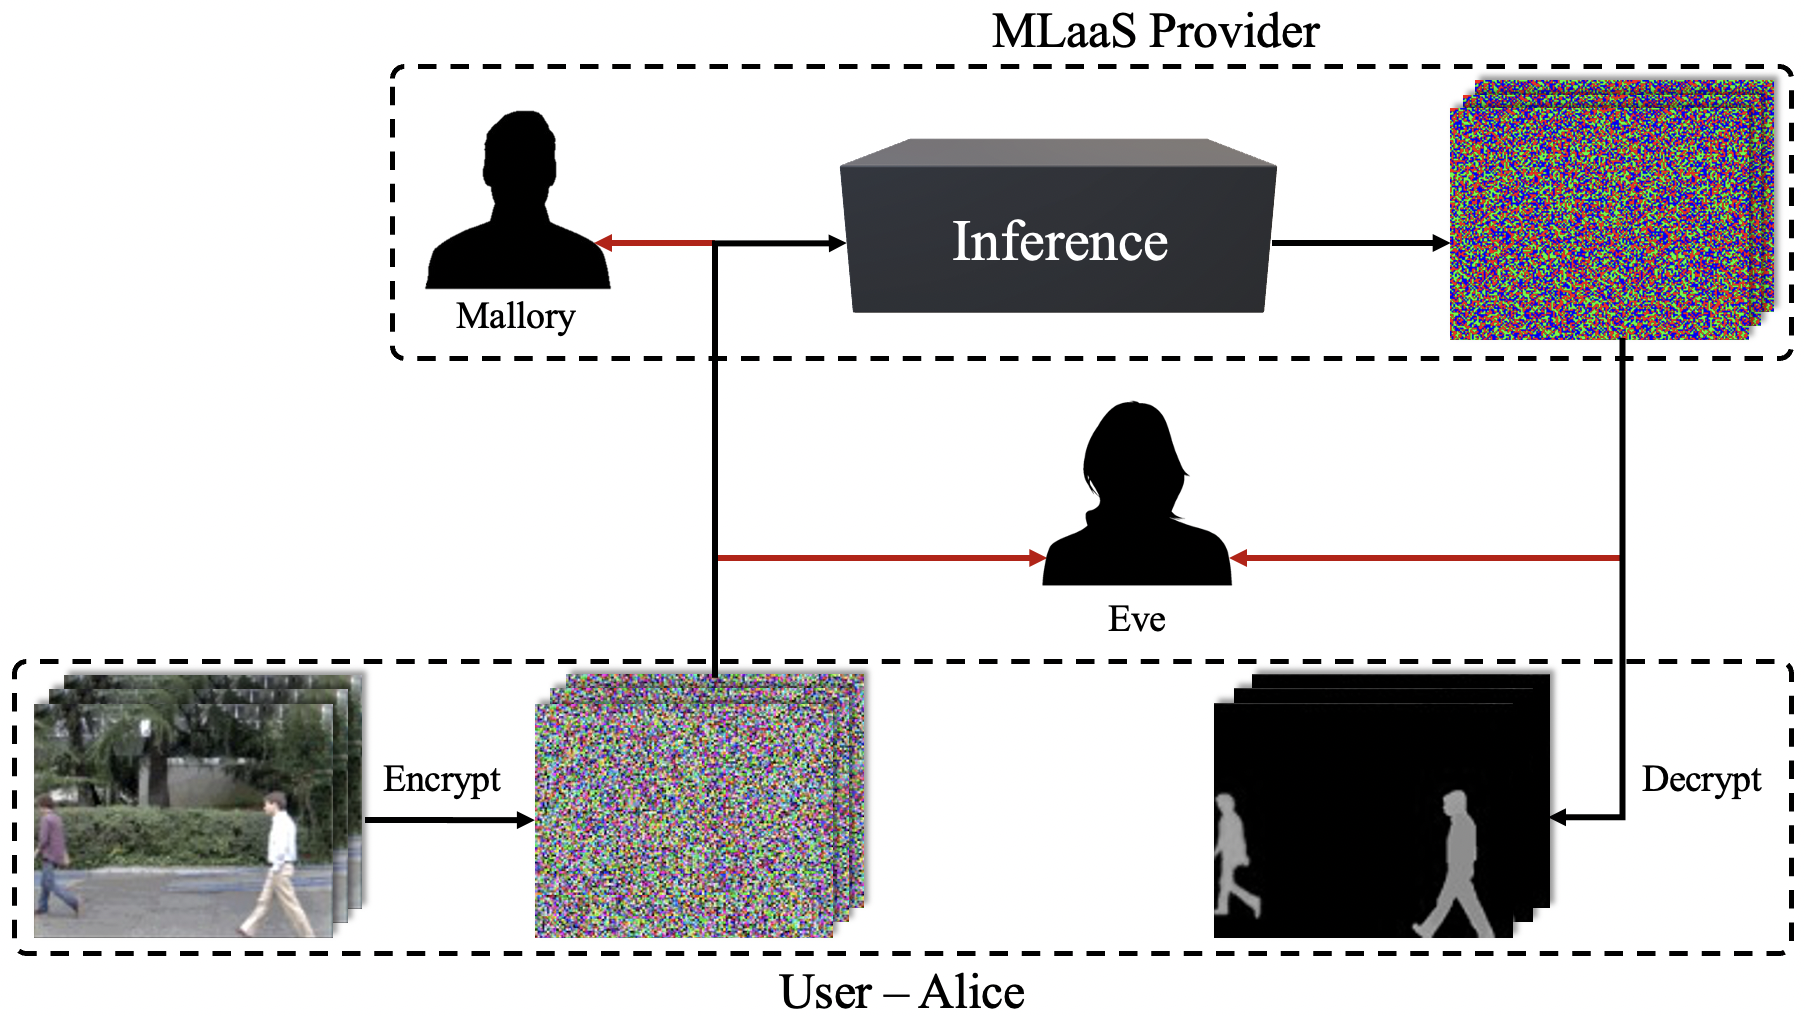
\includegraphics[width=0.8\textwidth]{figures/threatModel}
    \caption[The Threat Model]{A graphical representation of the threat model. Eve is an eavesdropper able to listen to communications between user and service provider. Mallory is a malicious actor within the service provider able to access users' video data. HE is able to obstruct both Eve and Mallory, preventing them from discovering the contents of the user's video.}
    \label{fig:threatModel}
\end{figure}






\section{Project Contributions}
\label{sec:projectContributions}
\indent \indent
This dissertation documents the design and implementation of a novel investigation into HE for video inference. It provides preliminary insight into the most challenging aspects of integrating the distinct fields of cryptography and computer vision to encourage further research. 
\begin{itemize}
    \item \textbf{Networking:} a client-server application simulating the device-server stack utilised by surveillance companies was constructed to enable the exploration of optimisations to increase the network throughput of videos encrypted using the CKKS HE scheme \cite{CKKS} provided by Microsoft's Secure Encrypted Arithmetic Library (SEAL) \cite{SEAL}.
    \item \textbf{Inference:} multiple inference algorithms were implemented to permit private and plain moving object detection, including investigating online GMMs following Stauffer and Grimson \cite{Stauffer} and the Expectation-Maximisation algorithm \cite{Dempster}.
    \item \textbf{MeKKS:} a HE implementation from first principles following the Homomorphic Encryption for Arithmetic of Approximate Numbers paper by Cheon et al.\ \cite{CKKS, BootstrappingHEAAN} to examine the benefits of specialising the implementation for video data by removing unneeded functionality, simplifying data structures, and vectorising ciphertexts.
\end{itemize}
